\documentclass{article}

% chinese fonts
\usepackage{ctex}

% math fonts
\usepackage{amsmath}
\usepackage{amsthm}
\usepackage{amssymb}
\usepackage{bm}

% figures
\usepackage{tikz}
\usepackage{graphicx}
\graphicspath{{./figures/}}

% tables
\usepackage{tabularx}
\usepackage{booktabs}
\usepackage{multirow}

% codes
\usepackage{listings}
\lstset{language     = Matlab,
        basicstyle   = \ttfamily,
        keywordstyle = \color{cyan},
        rulecolor    = \color{black},
        commentstyle = \color{green},
        keepspaces   = true,
        tabsize      = 4,
}

% hyperlinks
\usepackage{hyperref}
\hypersetup{
  breaklinks,
  colorlinks = true,
  citecolor  = blue,
  linkcolor  = red,
  urlcolor   = magenta,
}

% algorithms
\usepackage{algorithm}
\usepackage{algorithmic}

% bibliography
\usepackage[sort&compress,numbers]{natbib}

% About:  Macros for Vector, Matrix, Tensor, Math Operator and Misc
% Author: Jingxuan Yang

% vectors
\newcommand{\va}{\bm{a}}       \newcommand{\vah}{\hat{\bm{a}}}        \newcommand{\ah}{\hat{a}}    \newcommand{\vat}{\tilde{\bm{a}}}       \newcommand{\at}{\tilde{a}}
\newcommand{\vb}{\bm{b}}       \newcommand{\vbh}{\hat{\bm{b}}}        \newcommand{\bh}{\hat{b}}    \newcommand{\vbt}{\tilde{\bm{b}}}       \newcommand{\bt}{\tilde{b}}
\newcommand{\vc}{\bm{c}}       \newcommand{\vch}{\hat{\bm{c}}}        \newcommand{\ch}{\hat{c}}    \newcommand{\vct}{\tilde{\bm{c}}}       \newcommand{\ct}{\tilde{c}}
\newcommand{\vd}{\bm{d}}       \newcommand{\vdh}{\hat{\bm{d}}}        \newcommand{\dhat}{\hat{d}}  \newcommand{\vdt}{\tilde{\bm{d}}}       \newcommand{\dt}{\tilde{d}}
\newcommand{\ve}{\bm{e}}       \newcommand{\veh}{\hat{\bm{e}}}        \newcommand{\eh}{\hat{e}}    \newcommand{\vet}{\tilde{\bm{e}}}       \newcommand{\et}{\tilde{e}}
\newcommand{\vf}{\bm{f}}       \newcommand{\vfh}{\hat{\bm{f}}}        \newcommand{\fh}{\hat{f}}    \newcommand{\vft}{\tilde{\bm{f}}}       \newcommand{\ft}{\tilde{f}}
\newcommand{\vg}{\bm{g}}       \newcommand{\vgh}{\hat{\bm{g}}}        \newcommand{\gh}{\hat{g}}    \newcommand{\vgt}{\tilde{\bm{g}}}       \newcommand{\gt}{\tilde{g}}
\newcommand{\vh}{\bm{h}}     \newcommand{\vhh}{\hat{\bm{h}}}        \newcommand{\hh}{\hat{h}}    \newcommand{\vht}{\tilde{\bm{h}}}       \newcommand{\htild}{\tilde{h}}
\newcommand{\vi}{\bm{i}}       \newcommand{\vih}{\hat{\bm{i}}}        \newcommand{\ih}{\hat{i}}    \newcommand{\vit}{\tilde{\bm{i}}}       \newcommand{\itild}{\tilde{i}}
\newcommand{\vj}{\bm{j}}       \newcommand{\vjh}{\hat{\bm{j}}}        \newcommand{\jh}{\hat{j}}    \newcommand{\vjt}{\tilde{\bm{j}}}       \newcommand{\jt}{\tilde{j}}
\newcommand{\vk}{\bm{k}}       \newcommand{\vkh}{\hat{\bm{k}}}        \newcommand{\kh}{\hat{k}}    \newcommand{\vkt}{\tilde{\bm{k}}}       \newcommand{\kt}{\tilde{k}}
\newcommand{\vl}{\bm{l}}       \newcommand{\vlh}{\hat{\bm{l}}}        \newcommand{\lh}{\hat{l}}    \newcommand{\vlt}{\tilde{\bm{l}}}       \newcommand{\lt}{\tilde{l}}
\newcommand{\vm}{\bm{m}}       \newcommand{\vmh}{\hat{\bm{m}}}        \newcommand{\mh}{\hat{m}}    \newcommand{\vmt}{\tilde{\bm{m}}}       \newcommand{\mt}{\tilde{m}}
\newcommand{\vn}{\bm{n}}       \newcommand{\vnh}{\hat{\bm{n}}}        \newcommand{\nh}{\hat{n}}    \newcommand{\vnt}{\tilde{\bm{n}}}       \newcommand{\nt}{\tilde{n}}
\newcommand{\vo}{\bm{o}}       \newcommand{\voh}{\hat{\bm{o}}}        \newcommand{\oh}{\hat{o}}    \newcommand{\vot}{\tilde{\bm{o}}}       \newcommand{\ot}{\tilde{o}}
\newcommand{\vp}{\bm{p}}       \newcommand{\vph}{\hat{\bm{p}}}        \newcommand{\ph}{\hat{p}}    \newcommand{\vpt}{\tilde{\bm{p}}}       \newcommand{\pt}{\tilde{p}}
\newcommand{\vq}{\bm{q}}       \newcommand{\vqh}{\hat{\bm{q}}}        \newcommand{\qh}{\hat{q}}    \newcommand{\vqt}{\tilde{\bm{q}}}       \newcommand{\qt}{\tilde{q}}
\newcommand{\vr}{\bm{r}}       \newcommand{\vrh}{\hat{\bm{r}}}        \newcommand{\rh}{\hat{r}}    \newcommand{\vrt}{\tilde{\bm{r}}}       \newcommand{\rt}{\tilde{r}}
\newcommand{\vs}{\bm{s}}       \newcommand{\vsh}{\hat{\bm{s}}}        \newcommand{\sh}{\hat{s}}    \newcommand{\vst}{\tilde{\bm{s}}}       \newcommand{\st}{\tilde{s}}
\newcommand{\vt}{\bm{t}}       \newcommand{\vth}{\hat{\bm{t}}}        \newcommand{\that}{\hat{t}}  \newcommand{\vtt}{\tilde{\bm{t}}}       \newcommand{\ttil}{\tilde{t}}
\newcommand{\vu}{\bm{u}}       \newcommand{\vuh}{\hat{\bm{u}}}        \newcommand{\uh}{\hat{u}}    \newcommand{\vut}{\tilde{\bm{u}}}       \newcommand{\ut}{\tilde{u}}
\newcommand{\vv}{\bm{v}}       \newcommand{\vvh}{\hat{\bm{v}}}        \newcommand{\vhat}{\hat{v}}    \newcommand{\vvt}{\tilde{\bm{v}}}       \newcommand{\vtild}{\tilde{v}}
\newcommand{\vw}{\bm{w}}       \newcommand{\vwh}{\hat{\bm{w}}}        \newcommand{\wh}{\hat{w}}    \newcommand{\vwt}{\tilde{\bm{w}}}       \newcommand{\wt}{\tilde{w}}
\newcommand{\vx}{\bm{x}}       \newcommand{\vxh}{\hat{\bm{x}}}        \newcommand{\xh}{\hat{x}}    \newcommand{\vxt}{\tilde{\bm{x}}}       \newcommand{\xt}{\tilde{x}}
\newcommand{\vy}{\bm{y}}       \newcommand{\vyh}{\hat{\bm{y}}}        \newcommand{\yh}{\hat{y}}    \newcommand{\vyt}{\tilde{\bm{y}}}       \newcommand{\yt}{\tilde{y}}
\newcommand{\vz}{\bm{z}}       \newcommand{\vzh}{\hat{\bm{z}}}        \newcommand{\zh}{\hat{z}}    \newcommand{\vzt}{\tilde{\bm{z}}}       \newcommand{\zt}{\tilde{z}}

\newcommand{\valpha}{\bm{\alpha}}
\newcommand{\vbeta}{\bm{\beta}}
\newcommand{\vgamma}{\bm{\gamma}}
\newcommand{\vtheta}{\bm{\theta}}
\newcommand{\vlambda}{\bm{\lambda}}
\newcommand{\vmu}{\bm{\mu}}
\newcommand{\vomega}{\bm{\omega}}

\newcommand{\mSigma}{\bm{\Sigma}}

\newcommand{\Fc}{\mathcal{F}}
\newcommand{\Xc}{\mathcal{X}}
\newcommand{\Yc}{\mathcal{Y}}
\newcommand{\Zc}{\mathcal{Z}}
\newcommand{\Gc}{\mathcal{G}}
\newcommand{\Hc}{\mathcal{H}}
\newcommand{\Dc}{\mathcal{D}}
\newcommand{\Cc}{\mathcal{C}}
\newcommand{\Rc}{\mathcal{R}}

% matrices
\newcommand{\ma}{\bm{A}}
\newcommand{\mb}{\bm{B}}
\newcommand{\md}{\bm{D}}
\newcommand{\mH}{\bm{H}}
\newcommand{\mE}{\bm{E}}
\newcommand{\mi}{\bm{I}}
\newcommand{\mk}{\bm{K}}
\newcommand{\ml}{\bm{L}}
\newcommand{\mn}{\bm{N}}
\newcommand{\mP}{\bm{P}}
\newcommand{\mq}{\bm{Q}}
\newcommand{\mr}{\bm{R}}
\newcommand{\mU}{\bm{u}}
\newcommand{\mv}{\bm{v}}
\newcommand{\mw}{\bm{W}}
\newcommand{\mx}{\bm{X}}
\newcommand{\my}{\bm{Y}}
\newcommand{\mz}{\bm{Z}}

% tensors
\newcommand{\tp}{\mathsf{P}}
\newcommand{\tu}{\mathsf{U}}
\newcommand{\tx}{\mathsf{X}}
\newcommand{\ty}{\mathsf{Y}}
\newcommand{\tz}{\mathsf{Z}}
\newcommand{\tw}{\mathsf{W}}
\newcommand{\tf}{\mathsf{F}}
\newcommand{\ta}{\mathsf{A}}
\renewcommand{\th}{\mathsf{H}}

% norms
\newcommand{\mynorm}[2]{\| {#1} \|_{#2}}
\newcommand{\norm}[2]{\mynorm{#1}{#2}}
\newcommand{\bignorm}[2]{\left\| {#1} \right\|_{#2}}
\newcommand{\norml}[1]{\mynorm{#1}{1}}
\newcommand{\bignorml}[1]{\bignorm{#1}{1}}
\newcommand{\infnorm}[1]{\mynorm{#1}{\infty}}
\newcommand{\biginfnorm}[1]{\bignorm{#1}{\infty}}
\newcommand{\oneinf}{\ell_{1,\infty}}
\newcommand{\onetwo}{\ell_{1,2}}
\newcommand{\oneinfnorm}[1]{\mynorm{#1}{1,\infty}}
\newcommand{\bigoneinf}[1]{\bignorm{#1}{1,\infty}}
\newcommand{\onetwonorm}[1]{\mynorm{#1}{1,2}}
\newcommand{\bigonetwo}[1]{\bignorm{#1}{1,2}}
\newcommand{\enorm}[1]{\mynorm{#1}{2}}
\newcommand{\bigenorm}[1]{\bignorm{#1}{2}}
\newcommand{\znorm}[1]{\mynorm{#1}{0}}
\newcommand{\bigznorm}[1]{\bignorm{#1}{0}}
\newcommand{\frob}[1]{\|{#1}\|_{\text{F}}}
\newcommand{\bigfrob}[1]{\bignorm{#1}{\text{F}}}
\newcommand{\grpnorm}[2]{\norm{#1}{\text{Gr}(#2)}}

% math operators
\DeclareMathOperator*{\argmin}{argmin}
\DeclareMathOperator*{\argmax}{argmax}
\DeclareMathOperator{\divg}{div}
\DeclareMathOperator{\dom}{dom}
\DeclareMathOperator{\interior}{int}
\DeclareMathOperator{\ri}{ri}
\DeclareMathOperator{\sgn}{sgn}
\DeclareMathOperator{\trace}{Tr}
\DeclareMathOperator{\diag}{diag}
\DeclareMathOperator{\rank}{rank}
\DeclareMathOperator{\range}{range}
\DeclareMathOperator{\vect}{vec}
\DeclareMathOperator{\prox}{prox}
\DeclareMathOperator{\intr}{int}
\DeclareMathOperator{\relint}{ri}

% misc
\newcommand{\gs}{\geqslant}
\newcommand{\ls}{\leqslant}
\newcommand{\set}[1]{\left\{ {#1}\right\}}

\newcommand{\defeq}{\ \stackrel{\text{def}}{=}\ }
\newcommand{\ip}[2]{\left\langle#1, #2\right\rangle}
\newcommand{\reals}{\mathbb{R}}
\newcommand{\complex}{\mathbb{C}}
\newcommand{\half}{\frac{1}{2}}

\newtheorem{theorem}{Theorem}
\newtheorem{lemma}[theorem]{Lemma}
\newtheorem{proposition}[theorem]{Proposition}
\newtheorem{remark}[theorem]{Remark}
\newtheorem{corollary}[theorem]{Corollary}
\newtheorem{definition}[theorem]{Definition}


\setlength{\oddsidemargin}{-0.25 in}
\setlength{\evensidemargin}{-0.25 in} 
\setlength{\topmargin}{-0.25in} 
\setlength{\textwidth}{7 in} 
\setlength{\textheight}{8.5 in}
\setlength{\headsep}{0.25 in} 
\setlength{\parindent}{0 in}
\setlength{\parskip}{0.1 in}

\newcommand{\homework}[5]{
  \pagestyle{myheadings} 
  \thispagestyle{plain}
  \newpage
  \setcounter{page}{1} 
  \setcounter{section}{#5} 
  \noindent
  \begin{center}
    \framebox{ 
      \vbox{
        \vspace{2mm} 
        \hbox to 6.28in { {\bf
        THU-70250043-0,~Pattern~Recognition~(Spring 2021) \hfill Homework: 9} }
        \vspace{6mm} 
        \hbox to 6.28in { {\Large \hfill #1 \hfill} }
        \vspace{6mm} 
        \hbox to 6.28in { {\it Lecturer: #2 \hfill} }
        \vspace{2mm} 
        \hbox to 6.28in { {\it \hspace{14mm} #3 \hfill} }
        \vspace{2mm} 
        \hbox to 6.28in { {\it Student: #4 \hfill} }
        \vspace{2mm} 
      } 
    }
  \end{center}
  \markboth{#1}{#1} 
  \vspace*{4mm} 
}

\begin{document}

\homework{Deep Learning 2}{Changshui Zhang
\hspace{5mm} {\tt zcs@mail.tsinghua.edu.cn}}{Hong Zhao \hspace{16mm} {\tt vzhao@tsinghua.edu.cn}}{Jingxuan Yang \hspace{10mm} {\tt yangjx20@mails.tsinghua.edu.cn}}{8}


\section*{Recurrent Neural Network (RNN)}

1. In this problem, you will implement a recurrent neural network which implements binary addition. The inputs are given as binary sequences, starting with the least significant binary digit. (It is easier to start from the least significant bit, just like how you did addition in grade school.) The sequences will be padded with at least one zero on the end. For instance, the problem
\begin{equation}
  110111+10010=1001001
\end{equation}
would be represented as:
\begin{itemize}
  \item \textbf{Input 1}: 1, 1, 1, 0, 1, 1, 0 
  \item \textbf{Input 2}: 0, 1, 0, 0, 1, 0, 0 
  \item \textbf{Correct output}: 1, 0, 0, 1, 0, 0, 1 
\end{itemize}

There are two input units corresponding to the two inputs, and one output unit. Therefore, the pattern of inputs and outputs for this example would be:
\begin{figure}[!ht]
   \centering
   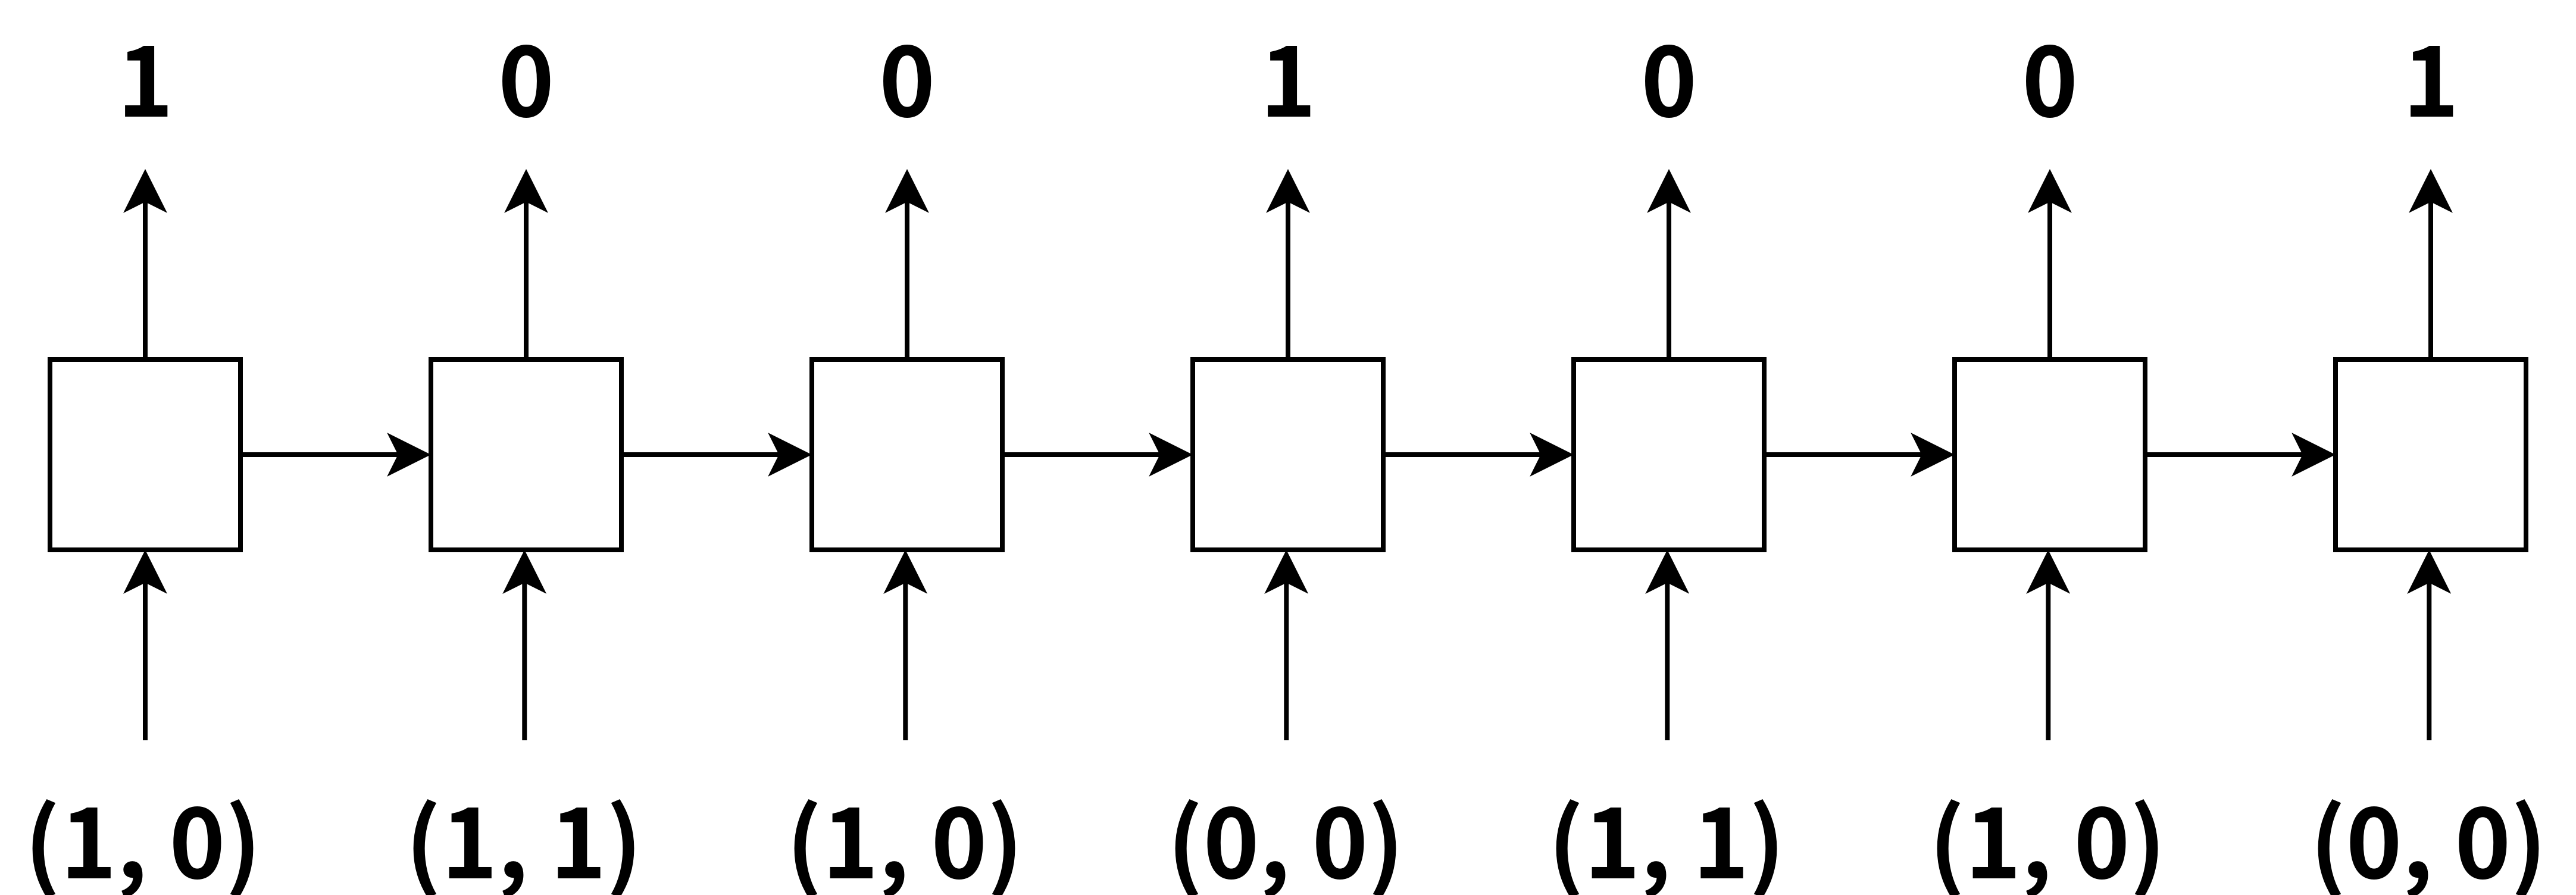
\includegraphics[scale=0.5]{fig1.png}
   \label{fig:1_1}
\end{figure}

Design the weights and biases for an RNN which has two input units, three hidden units, and one output unit, which implements binary addition. All the units use the hard threshold activation function. In particular, specify the values of weight matrices \(\bm{U}, \bm{V},\) and \(\bm{W},\) bias vector \(\bm{b}_{\bm{h}},\) and scalar bias \(b_{y}\). The details of the architecture and the computation are as follows:
\begin{figure}[!ht]
   \centering
   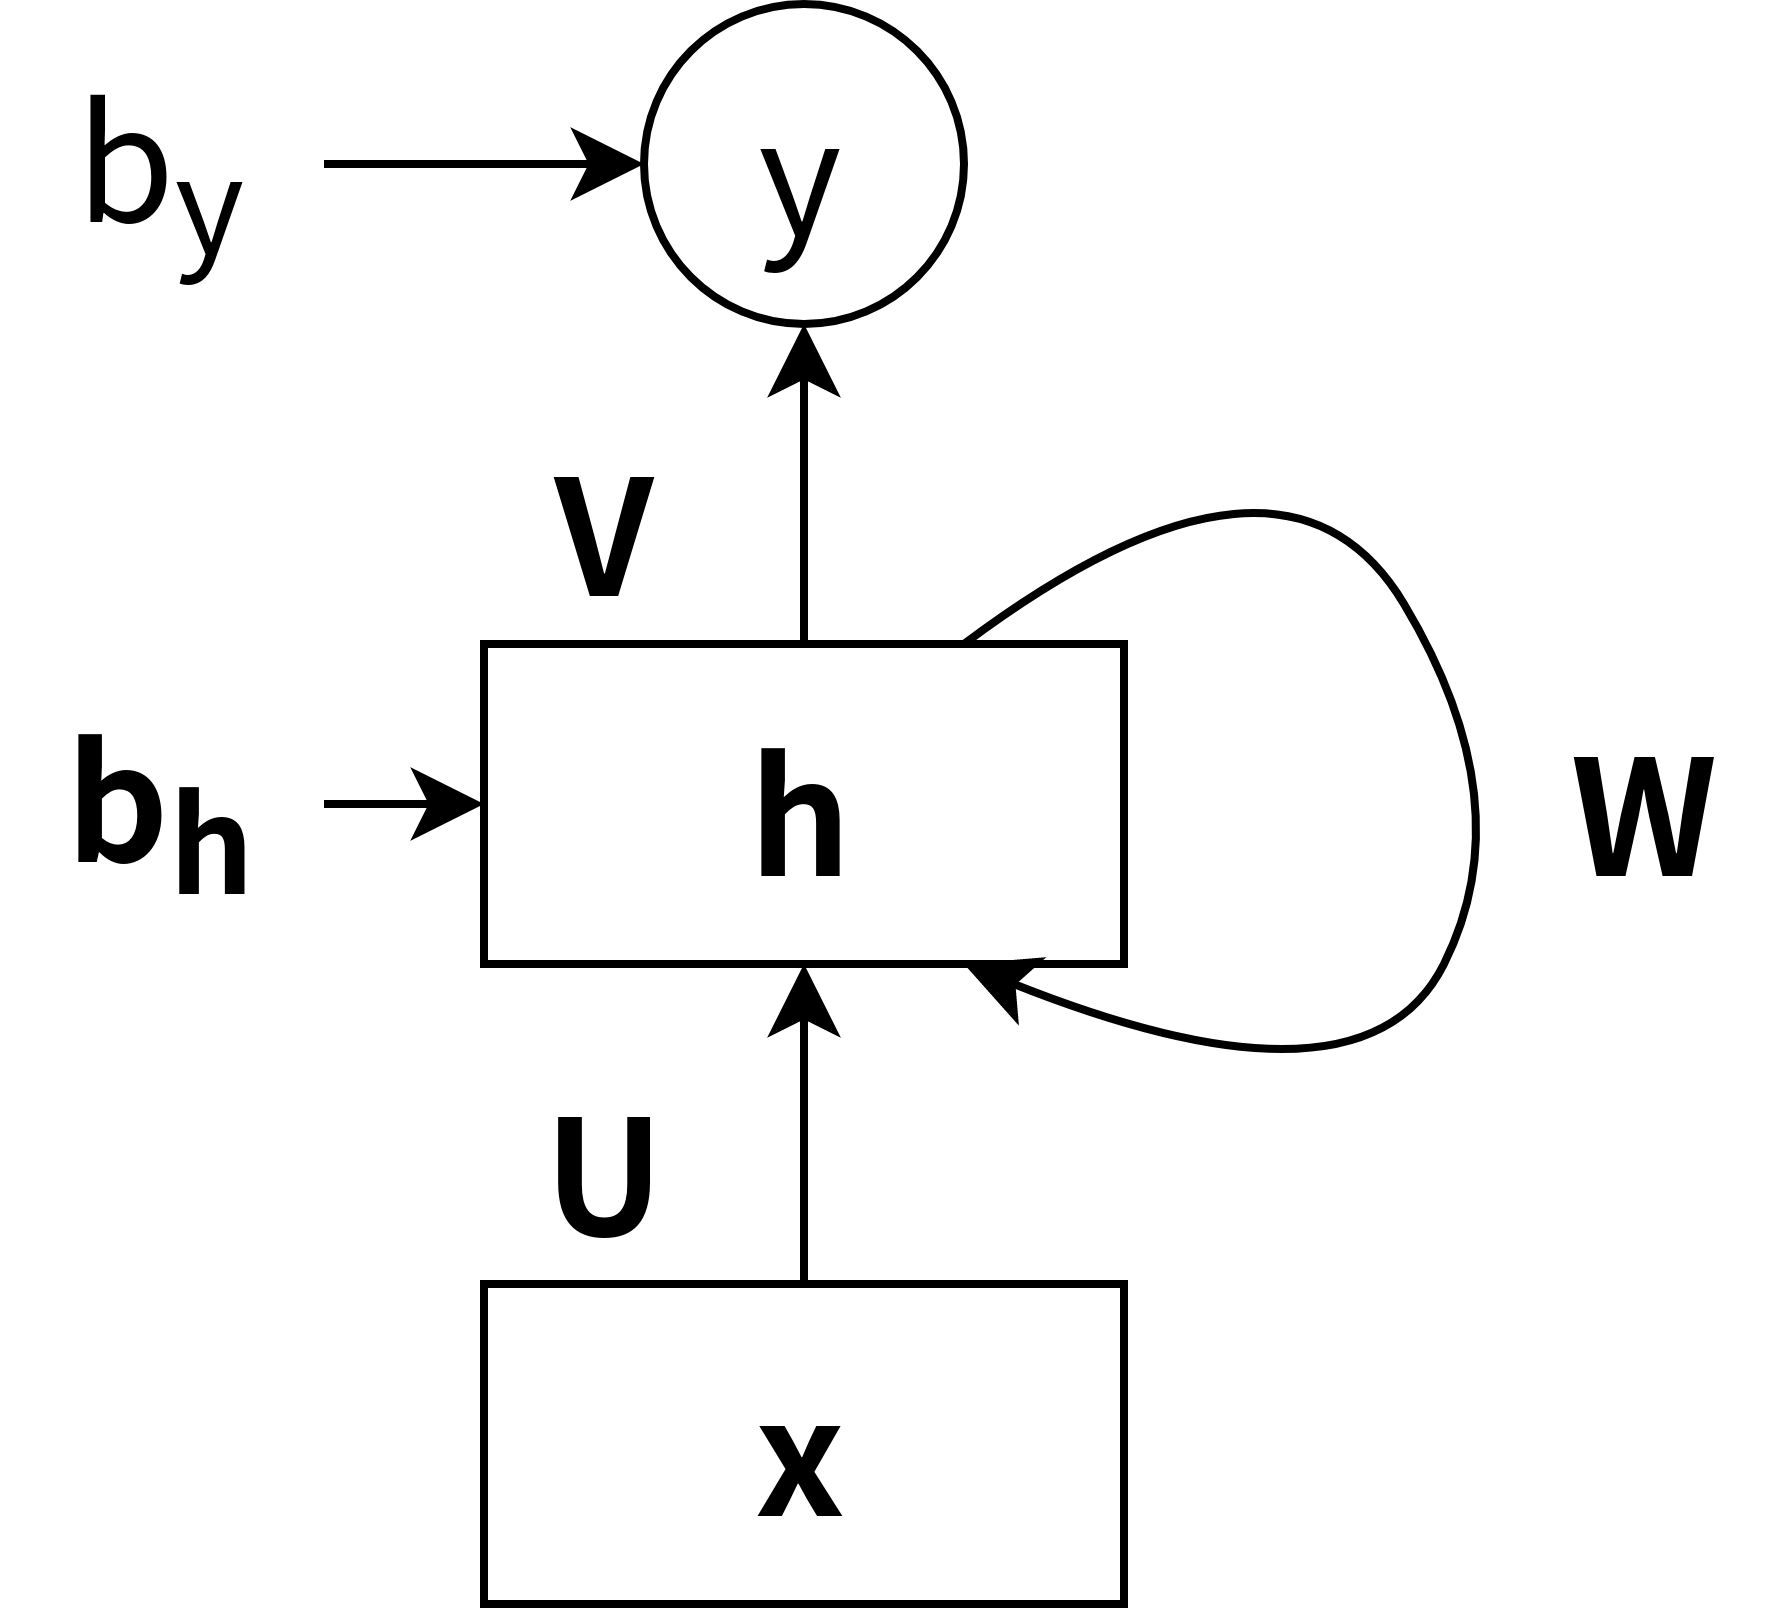
\includegraphics[scale=0.5]{fig2.png}
   \label{fig:1_2}
\end{figure}
\begin{equation}
  \begin{aligned}
    \bm{h}^{(t)} &= \mathrm{hard}(\bm{U}\bm{x}^{(t)} + \bm{W}\bm{h}^{(t-1)} + \bm{b}_{\bm{h}}) \\
    y^{(t)} &= \mathrm{hard}(\bm{V}\bm{h}^{(t)} + b_{y}) \\
  \end{aligned}
\end{equation}
\begin{equation}
  \mathrm{hard}(x)=
  \begin{cases}
    0, &\text{if}~x<0 \\
    1, &\text{if}~x\gs0 \\
  \end{cases}
\end{equation}

If $\bm{x}$ is a vector, $\mathrm{hard}(\bm{x})$ represents element-wise operation. And we initialize $\bm{h}^{(0)}$ as $\bm{0}$.

\emph{Hint}: One simple implementation of the first layer is that you just add up the values of each unit, including the carry. Activate the first one of your hidden units if the sum is at least 1, the second one if it is at least 2, and the third one if it is 3. Obviously, the answer is not unique, and you are encouraged to find more interesting implementation, but one is enough for this homework.

解: 根据提示, 可设计 RNN 如下.
\begin{equation}
  \mU=\begin{bmatrix}
    1 & 1 \\
    1 & 1 \\
    1 & 1 \\
  \end{bmatrix},\quad
  \mv=\begin{bmatrix}
    1 & -1 & 1 \\
  \end{bmatrix},\quad
  \mw=\frac{1}{2}\begin{bmatrix}
    1 & 1 & 1 \\
    1 & 1 & 1 \\
    1 & 1 & 1 \\
  \end{bmatrix},\quad
  \vb_{\vh}=\begin{bmatrix}
    -1 \\ -2 \\ -3 \\
  \end{bmatrix},\quad
  b_y=-\frac{1}{2}
\end{equation}

初始化 $\vh^{(0)}=\bm{0}$, 对于示例题目可计算如下. 输入为
\begin{equation}
  \vx=\begin{bmatrix}
    1 & 1 & 1 & 0 & 1 & 1 & 0 \\
    0 & 1 & 0 & 0 & 1 & 0 & 0 \\
  \end{bmatrix}
\end{equation}

正确输出为
\begin{equation}
  \vy=\begin{bmatrix}
    1 & 0 & 0 & 1 & 0 & 0 & 1 \\
  \end{bmatrix}
\end{equation}

第 1 步计算:
\begin{equation}
  \vh^{(1)}
  =\hard\left(
    \begin{bmatrix}
      1 & 1 \\
      1 & 1 \\
      1 & 1 \\
    \end{bmatrix}
    \begin{bmatrix}
      1 \\ 0 \\
    \end{bmatrix}
    +\frac{1}{2}
    \begin{bmatrix}
      1 & 1 & 1 \\
      1 & 1 & 1 \\
      1 & 1 & 1 \\
    \end{bmatrix}
    \begin{bmatrix}
      0 \\ 0 \\ 0 \\
    \end{bmatrix}
    +
    \begin{bmatrix}
      -1 \\ -2 \\ -3 \\
    \end{bmatrix}
  \right)
  =\hard\left(
    \begin{bmatrix}
      0 \\ -1 \\ -2 \\
    \end{bmatrix}
  \right)
  =
  \begin{bmatrix}
    1 \\ 0 \\ 0 \\
  \end{bmatrix}
\end{equation}

\begin{equation}
  y^{(1)}
  =\hard\left(
    \begin{bmatrix}
      1 & -1 & 1 \\
    \end{bmatrix}
    \begin{bmatrix}
      1 \\ 0 \\ 0 \\
    \end{bmatrix}
    -\frac{1}{2}
  \right)
  =\hard\left(
    \frac{1}{2}
  \right)
  =1
\end{equation}

第 2 步计算:
\begin{equation}
  \vh^{(2)}
  =\hard\left(
    \begin{bmatrix}
      1 & 1 \\
      1 & 1 \\
      1 & 1 \\
    \end{bmatrix}
    \begin{bmatrix}
      1 \\ 1 \\
    \end{bmatrix}
    +\frac{1}{2}
    \begin{bmatrix}
      1 & 1 & 1 \\
      1 & 1 & 1 \\
      1 & 1 & 1 \\
    \end{bmatrix}
    \begin{bmatrix}
      1 \\ 0 \\ 0 \\
    \end{bmatrix}
    +
    \begin{bmatrix}
      -1 \\ -2 \\ -3 \\
    \end{bmatrix}
  \right)
  =\hard\left(
    \begin{bmatrix}
      3/2 \\ 1/2 \\ -1/2 \\
    \end{bmatrix}
  \right)
  =
  \begin{bmatrix}
    1 \\ 1 \\ 0 \\
  \end{bmatrix}
\end{equation}

\begin{equation}
  y^{(2)}
  =\hard\left(
    \begin{bmatrix}
      1 & -1 & 1 \\
    \end{bmatrix}
    \begin{bmatrix}
      1 \\ 1 \\ 0 \\
    \end{bmatrix}
    -\frac{1}{2}
  \right)
  =\hard\left(
    -\frac{1}{2}
  \right)
  =0
\end{equation}

第 3 步计算:
\begin{equation}
  \vh^{(3)}
  =\hard\left(
    \begin{bmatrix}
      1 & 1 \\
      1 & 1 \\
      1 & 1 \\
    \end{bmatrix}
    \begin{bmatrix}
      1 \\ 0 \\
    \end{bmatrix}
    +\frac{1}{2}
    \begin{bmatrix}
      1 & 1 & 1 \\
      1 & 1 & 1 \\
      1 & 1 & 1 \\
    \end{bmatrix}
    \begin{bmatrix}
      1 \\ 1 \\ 0 \\
    \end{bmatrix}
    +
    \begin{bmatrix}
      -1 \\ -2 \\ -3 \\
    \end{bmatrix}
  \right)
  =\hard\left(
    \begin{bmatrix}
      1 \\ 0 \\ -1 \\
    \end{bmatrix}
  \right)
  =
  \begin{bmatrix}
    1 \\ 1 \\ 0 \\
  \end{bmatrix}
\end{equation}

\begin{equation}
  y^{(3)}
  =\hard\left(
    \begin{bmatrix}
      1 & -1 & 1 \\
    \end{bmatrix}
    \begin{bmatrix}
      1 \\ 1 \\ 0 \\
    \end{bmatrix}
    -\frac{1}{2}
  \right)
  =\hard\left(
    -\frac{1}{2}
  \right)
  =0
\end{equation}

第 4 步计算:
\begin{equation}
  \vh^{(4)}
  =\hard\left(
    \begin{bmatrix}
      1 & 1 \\
      1 & 1 \\
      1 & 1 \\
    \end{bmatrix}
    \begin{bmatrix}
      0 \\ 0 \\
    \end{bmatrix}
    +\frac{1}{2}
    \begin{bmatrix}
      1 & 1 & 1 \\
      1 & 1 & 1 \\
      1 & 1 & 1 \\
    \end{bmatrix}
    \begin{bmatrix}
      1 \\ 1 \\ 0 \\
    \end{bmatrix}
    +
    \begin{bmatrix}
      -1 \\ -2 \\ -3 \\
    \end{bmatrix}
  \right)
  =\hard\left(
    \begin{bmatrix}
      0 \\ -1 \\ -2 \\
    \end{bmatrix}
  \right)
  =
  \begin{bmatrix}
    1 \\ 0 \\ 0 \\
  \end{bmatrix}
\end{equation}

\begin{equation}
  y^{(4)}
  =\hard\left(
    \begin{bmatrix}
      1 & -1 & 1 \\
    \end{bmatrix}
    \begin{bmatrix}
      1 \\ 0 \\ 0 \\
    \end{bmatrix}
    -\frac{1}{2}
  \right)
  =\hard\left(
    \frac{1}{2}
  \right)
  =1
\end{equation}

第 5 步计算:
\begin{equation}
  \vh^{(5)}
  =\hard\left(
    \begin{bmatrix}
      1 & 1 \\
      1 & 1 \\
      1 & 1 \\
    \end{bmatrix}
    \begin{bmatrix}
      1 \\ 1 \\
    \end{bmatrix}
    +\frac{1}{2}
    \begin{bmatrix}
      1 & 1 & 1 \\
      1 & 1 & 1 \\
      1 & 1 & 1 \\
    \end{bmatrix}
    \begin{bmatrix}
      1 \\ 0 \\ 0 \\
    \end{bmatrix}
    +
    \begin{bmatrix}
      -1 \\ -2 \\ -3 \\
    \end{bmatrix}
  \right)
  =\hard\left(
    \begin{bmatrix}
      3/2 \\ 1/2 \\ -1/2 \\
    \end{bmatrix}
  \right)
  =
  \begin{bmatrix}
    1 \\ 1 \\ 0 \\
  \end{bmatrix}
\end{equation}

\begin{equation}
  y^{(5)}
  =\hard\left(
    \begin{bmatrix}
      1 & -1 & 1 \\
    \end{bmatrix}
    \begin{bmatrix}
      1 \\ 1 \\ 0 \\
    \end{bmatrix}
    -\frac{1}{2}
  \right)
  =\hard\left(
    -\frac{1}{2}
  \right)
  =0
\end{equation}

第 6 步计算:
\begin{equation}
  \vh^{(6)}
  =\hard\left(
    \begin{bmatrix}
      1 & 1 \\
      1 & 1 \\
      1 & 1 \\
    \end{bmatrix}
    \begin{bmatrix}
      1 \\ 0 \\
    \end{bmatrix}
    +\frac{1}{2}
    \begin{bmatrix}
      1 & 1 & 1 \\
      1 & 1 & 1 \\
      1 & 1 & 1 \\
    \end{bmatrix}
    \begin{bmatrix}
      1 \\ 1 \\ 0 \\
    \end{bmatrix}
    +
    \begin{bmatrix}
      -1 \\ -2 \\ -3 \\
    \end{bmatrix}
  \right)
  =\hard\left(
    \begin{bmatrix}
      1 \\ 0 \\ -1 \\
    \end{bmatrix}
  \right)
  =
  \begin{bmatrix}
    1 \\ 1 \\ 0 \\
  \end{bmatrix}
\end{equation}

\begin{equation}
  y^{(6)}
  =\hard\left(
    \begin{bmatrix}
      1 & -1 & 1 \\
    \end{bmatrix}
    \begin{bmatrix}
      1 \\ 1 \\ 0 \\
    \end{bmatrix}
    -\frac{1}{2}
  \right)
  =\hard\left(
    -\frac{1}{2}
  \right)
  =0
\end{equation}

第 7 步计算:
\begin{equation}
  \vh^{(7)}
  =\hard\left(
    \begin{bmatrix}
      1 & 1 \\
      1 & 1 \\
      1 & 1 \\
    \end{bmatrix}
    \begin{bmatrix}
      0 \\ 0 \\
    \end{bmatrix}
    +\frac{1}{2}
    \begin{bmatrix}
      1 & 1 & 1 \\
      1 & 1 & 1 \\
      1 & 1 & 1 \\
    \end{bmatrix}
    \begin{bmatrix}
      1 \\ 1 \\ 0 \\
    \end{bmatrix}
    +
    \begin{bmatrix}
      -1 \\ -2 \\ -3 \\
    \end{bmatrix}
  \right)
  =\hard\left(
    \begin{bmatrix}
      0 \\ -1 \\ -2 \\
    \end{bmatrix}
  \right)
  =
  \begin{bmatrix}
    1 \\ 0 \\ 0 \\
  \end{bmatrix}
\end{equation}

\begin{equation}
  y^{(7)}
  =\hard\left(
    \begin{bmatrix}
      1 & -1 & 1 \\
    \end{bmatrix}
    \begin{bmatrix}
      1 \\ 0 \\ 0 \\
    \end{bmatrix}
    -\frac{1}{2}
  \right)
  =\hard\left(
    \frac{1}{2}
  \right)
  =1
\end{equation}

由于
\begin{equation}
  \vy
  =\begin{bmatrix}
    1 & 0 & 0 & 1 & 0 & 0 & 1 \\
  \end{bmatrix}
  =\begin{bmatrix}
    y^{(1)} & y^{(2)} & y^{(3)} & y^{(4)} & y^{(5)} & y^{(6)} & y^{(7)} \\
  \end{bmatrix}
\end{equation}

则上述设计的 RNN 可以实现二进制加法.

\section*{Long-Term Short-Term Memory (LSTM)}

2. Here, you'll derive the Backprop Through Time (BPTT) equations for the univariate version of the Long-Term Short-Term Memory (LSTM) architecture.

\emph{Note}: This question is an important context for understanding LSTMs, but it is just ordinary BPTT, so you have enough knowledge to do parts (a), (b). As for parts (c), you may find it helpful to read more materials about LSTM.

For reference, here are the computations it performs for inputs $x^{(t)}$, $t=1,2,\dots,T$:
\begin{equation}
  \begin{aligned}
      i^{(t)}&=\sigma\left(w_{i x} x^{(t)}+w_{i h} h^{(t-1)}\right) \\ 
      f^{(t)}&=\sigma\left(w_{f x} x^{(t)}+w_{f h} h^{(t-1)}\right) \\ 
      o^{(t)}&=\sigma\left(w_{o x} x^{(t)}+w_{o h} h^{(t-1)}\right) \\ 
      g^{(t)}&=\tanh\left(w_{g x} x^{(t)}+w_{g h} h^{(t-1)}\right) \\ 
      c^{(t)}&=f^{(t)} c^{(t-1)}+i^{(t)}g^{(t)} \\ 
      h^{(t)}&=o^{(t)}\tanh\left(c^{(t)}\right)\\
  \end{aligned}
\end{equation}

And the loss function $\mathcal{L}$ with label $y$ is:
\begin{equation}
  \mathcal{L} = \frac{1}{2}\left(y-h^{(T)}\right)^2
\end{equation}

A slightly more convenient notation:
\begin{itemize}
  \item $\sigma$ is the activation function, we use Sigmoid function here. 
  \item Use $\bar{y}$ to denote the derivative $\partial\mathcal{L}/\partial y$, sometimes called the error signal, where $\mathcal{L}$ is the loss function, $y$ can be any intermediate variable. This emphasizes that the error signals are just values our program is computing rather than a mathematical operation.
  \item As an example, we compute the loss:
  \begin{equation}
    \begin{aligned}
      z &= wx + b\\
      y &= \sigma(z)\\
      \mathcal{L} &= \frac{1}{2}(y-y_\mathrm{pred})^2 \\
    \end{aligned}
  \end{equation}
  Then we could compute the derivatives:
  \begin{equation}
    \bar{y} = y - y_\mathrm{pred},\quad
    \bar{z} = \bar{y}\sigma'(z),\quad
    \bar{w} = \bar{z}x,\quad
    \bar{b} = \bar{z}
  \end{equation}
  \item You should use this notation in the following questions.
\end{itemize}

Suppose that $T = 2$, and the initial values of $h^{(0)}$ and $c^{(0)}$ are known.

(a) Derive the Backprop Through Time equations for the activations and the gates for $t=1, 2$.
\begin{equation}
  \overline{h^{(t)}},\quad
  \overline{c^{(t)}},\quad
  \overline{o^{(t)}},\quad
  \overline{g^{(t)}},\quad
  \overline{i^{(t)}},\quad
  \overline{f^{(t)}}.
\end{equation}

解: 由于本题是单变量 (univariate) 版本 LSTM, 即全部变量为实数, 故将 $\odot$ 省略. 

由 $T=2$ 可知损失函数 $\Lc$ 为
\begin{equation}
  \Lc=\frac{1}{2}\left(y-h^{(2)}\right)^2
\end{equation}

所以, 损失函数 $\Lc$ 对 $h^{(2)}$ 的偏导数为
\begin{equation}
  \overline{h^{(2)}}
  =\frac{\partial\Lc}{\partial h^{(2)}}
  =h^{(2)}-y
\end{equation}

损失函数 $\Lc$ 对 $c^{(2)}$ 的偏导数为
\begin{equation}
    \overline{c^{(2)}}
    =\frac{\partial\Lc}{\partial c^{(2)}}
    =\frac{\partial\Lc}{\partial h^{(2)}}\frac{\partial h^{(2)}}{\partial c^{(2)}}
    =\overline{h^{(2)}}o^{(2)}\left[1-\tanh^2\left(c^{(2)}\right)\right]
\end{equation}

损失函数 $\Lc$ 对 $o^{(2)}$ 的偏导数为
\begin{equation}
    \overline{o^{(2)}}
    =\frac{\partial\Lc}{\partial o^{(2)}}
    =\frac{\partial\Lc}{\partial h^{(2)}}\frac{\partial h^{(2)}}{\partial o^{(2)}}
    =\overline{h^{(2)}}\tanh\left(c^{(2)}\right)
\end{equation}

损失函数 $\Lc$ 对 $g^{(2)}$ 的偏导数为
\begin{equation}
    \overline{g^{(2)}}
    =\frac{\partial\Lc}{\partial g^{(2)}}
    =\frac{\partial\Lc}{\partial c^{(2)}}\frac{\partial c^{(2)}}{\partial g^{(2)}}
    =\overline{c^{(2)}}i^{(2)}
\end{equation}

损失函数 $\Lc$ 对 $i^{(2)}$ 的偏导数为
\begin{equation}
    \overline{i^{(2)}}
    =\frac{\partial\Lc}{\partial i^{(2)}}
    =\frac{\partial\Lc}{\partial c^{(2)}}\frac{\partial c^{(2)}}{\partial i^{(2)}}
    =\overline{c^{(2)}}g^{(2)}
\end{equation}

损失函数 $\Lc$ 对 $f^{(2)}$ 的偏导数为
\begin{equation}
    \overline{f^{(2)}}
    =\frac{\partial\Lc}{\partial f^{(2)}}
    =\frac{\partial\Lc}{\partial c^{(2)}}\frac{\partial c^{(2)}}{\partial f^{(2)}}
    =\overline{c^{(2)}}c^{(1)}
\end{equation}

损失函数 $\Lc$ 对 $h^{(1)}$ 的偏导数为
\begin{equation}
  \begin{aligned}
    \overline{h^{(1)}}
    &=\frac{\partial\Lc}{\partial h^{(1)}}\\
    &=\frac{\partial\Lc}{\partial i^{(2)}}\frac{\partial i^{(2)}}{\partial h^{(1)}}
      +\frac{\partial\Lc}{\partial f^{(2)}}\frac{\partial f^{(2)}}{\partial h^{(1)}}
      +\frac{\partial\Lc}{\partial o^{(2)}}\frac{\partial o^{(2)}}{\partial h^{(1)}}
      +\frac{\partial\Lc}{\partial g^{(2)}}\frac{\partial g^{(2)}}{\partial h^{(1)}}\\
    &=\overline{i^{(2)}}i^{(2)}(1-i^{(2)})w_{ih}+\overline{f^{(2)}}f^{(2)}(1-f^{(2)})w_{fh}+\overline{o^{(2)}}o^{(2)}(1-o^{(2)})w_{oh}+\overline{g^{(2)}}[1-(g^{(2)})^2]w_{gh}\\
  \end{aligned}
\end{equation}

损失函数 $\Lc$ 对 $c^{(1)}$ 的偏导数为
\begin{equation}
  \begin{aligned}
    \overline{c^{(1)}}
    &=\frac{\partial\Lc}{\partial c^{(1)}}\\
    &=\frac{\partial\Lc}{\partial c^{(2)}}\frac{\partial c^{(2)}}{\partial c^{(1)}}
      +\frac{\partial\Lc}{\partial h^{(1)}}\frac{\partial h^{(1)}}{\partial c^{(1)}}\\
    &=\overline{c^{(2)}}f^{(2)}
      +\overline{h^{(1)}}o^{(1)}\left[1-\tanh^2\left(c^{(1)}\right)\right]\\
  \end{aligned}
\end{equation}

损失函数 $\Lc$ 对 $o^{(1)}$ 的偏导数为
\begin{equation}
    \overline{o^{(1)}}
    =\frac{\partial\Lc}{\partial o^{(1)}}
    =\frac{\partial\Lc}{\partial h^{(1)}}\frac{\partial h^{(1)}}{\partial o^{(1)}}
    =\overline{h^{(1)}}\tanh\left(c^{(1)}\right)
\end{equation}

损失函数 $\Lc$ 对 $g^{(1)}$ 的偏导数为
\begin{equation}
    \overline{g^{(1)}}
    =\frac{\partial\Lc}{\partial g^{(1)}}
    =\frac{\partial\Lc}{\partial c^{(1)}}\frac{\partial c^{(1)}}{\partial g^{(1)}}
    =\overline{c^{(1)}}i^{(1)}
\end{equation}

损失函数 $\Lc$ 对 $i^{(1)}$ 的偏导数为
\begin{equation}
    \overline{i^{(1)}}
    =\frac{\partial\Lc}{\partial i^{(1)}}
    =\frac{\partial\Lc}{\partial c^{(1)}}\frac{\partial c^{(1)}}{\partial i^{(1)}}
    =\overline{c^{(1)}}g^{(1)}
\end{equation}

损失函数 $\Lc$ 对 $f^{(1)}$ 的偏导数为
\begin{equation}
    \overline{f^{(1)}}
    =\frac{\partial\Lc}{\partial f^{(1)}}
    =\frac{\partial\Lc}{\partial c^{(1)}}\frac{\partial c^{(1)}}{\partial f^{(1)}}
    =\overline{c^{(1)}}c^{(0)}
\end{equation}

(b) Derive the Backprop Through Time equation for the weight $w_{ix}$. (The other weight matrices are basically the same, so we won't make you write those out.)

解: 损失函数 $\Lc$ 对 $w_{ix}$ 的偏导数为
\begin{equation}
  \begin{aligned}
    \overline{w_{ix}}
    &=\frac{\partial\Lc}{\partial w_{ix}}\\
    &=\frac{\partial\Lc}{\partial i^{(2)}}\frac{\partial i^{(2)}}{\partial w_{ix}}
      +\frac{\partial\Lc}{\partial i^{(1)}}\frac{\partial i^{(1)}}{\partial w_{ix}}\\
    &=\overline{i^{(2)}}i^{(2)}(1-i^{(2)})x^{(2)}+\overline{i^{(1)}}i^{(1)}(1-i^{(1)})x^{(1)}\\
  \end{aligned}
\end{equation}

(c) (\emph{Optional}) Based on your answers above, can you explain why the gradient doesn't explode if the values of the forget gates ($f^{(t)}$) are very close to 1 and the values of the input and output gates ($i^{(t)}$ and $o^{(t)}$) are very close to 0? (Your answer may involve both $\overline{h^{(t)}}$ and $\overline{c^{(t)}}$.)

解: 由 $f^{(t)}\approx1$, $o^{(t)}\approx0$, $\forall~t=1,2,\dots,T$ 可知
\begin{equation}
  \overline{c^{(t)}}
  =\overline{c^{(t+1)}}f^{(t+1)}
   +\overline{h^{(t)}}o^{(t)}\left[1-\tanh^2\left(c^{(t)}\right)\right]
  \approx\overline{c^{(t+1)}},\quad\forall~t=1,2,\dots,T-1
\end{equation}

所以
\begin{equation}
  \overline{c^{(t)}}\approx\overline{c^{(T)}},\quad\forall~t=1,2,\dots,T-1
\end{equation}

损失函数 $\Lc$ 对 $w_{ix}$ 的偏导数为
\begin{equation}
  \begin{aligned}
    \overline{w_{ix}}
    &=\sum_{t=1}^T\overline{i^{(t)}}i^{(t)}(1-i^{(t)})x^{(t)}\\
    &=\sum_{t=1}^T\overline{c^{(t)}}g^{(t)}i^{(t)}(1-i^{(t)})x^{(t)}\\
    &\approx\sum_{t=1}^T\overline{c^{(T)}}g^{(t)}i^{(t)}(1-i^{(t)})x^{(t)}\\
    &=\sum_{t=1}^T\overline{h^{(T)}}\left[1-\tanh^2\left(c^{(T)}\right)\right]g^{(t)}i^{(t)}(1-i^{(t)})x^{(t)}\\
    &=\sum_{t=1}^T(h^{(T)}-y)\left[1-\tanh^2\left(c^{(T)}\right)\right]g^{(t)}i^{(t)}(1-i^{(t)})x^{(t)}\\
  \end{aligned}
\end{equation}

注意到 $i^{(t)}\approx0$, $\forall~t=1,2,\dots,T$, 对 $|\overline{w_{ix}}|$ 估计其上界得
\begin{equation}
  \begin{aligned}
    |\overline{w_{ix}}|
    &=|h^{(T)}-y|\left[1-\tanh^2\left(c^{(T)}\right)\right]\left|\sum_{t=1}^Tg^{(t)}i^{(t)}(1-i^{(t)})x^{(t)}\right|\\
    &\ls|h^{(T)}-y|\left[1-\tanh^2\left(c^{(T)}\right)\right]\sum_{t=1}^Tg^{(t)}i^{(t)}(1-i^{(t)})|x^{(t)}|\\
    &\ls(1+|y|)\sum_{t=1}^Ti^{(t)}(1-i^{(t)})\max_{1\ls t\ls T}|x^{(t)}|\\
    &=(1+|y|)\max_{1\ls t\ls T}|x^{(t)}|\sum_{t=1}^Ti^{(t)}(1-i^{(t)})\\
    &\approx0
  \end{aligned}
\end{equation}

因此梯度 $\overline{w_{ix}}$ 并不会爆炸.

\section*{Attention}

3. Recall that attention can be viewed as an operation on a query $\vq\in\mathbb{R}^{d}$, a set of value vectors $\{\vv_{1},\vv_2, \dots, \vv_{n}\}$, $\vv_{i} \in \mathbb{R}^{d}$, and a set of key vectors $\{\vk_{1},\vk_2,\dots, \vk_{n}\}$, $\vk_{i} \in \mathbb{R}^{d}$, specified as follows:
\begin{equation}
   \vc=\sum_{i=1}^{n} \alpha_{i}\vv_{i} 
\end{equation} 
\begin{equation}
  \alpha_{i}
  =\frac{\exp(\vk_{i}^{\top}\vq)}{\sum_{j=1}^{n}\exp(\vk_{j}^{\top}\vq)}
\end{equation}
where $\alpha_i$ are frequently called the ``attention weights'', and the output $\vc \in \mathbb{R}^{d}$ is a correspondingly weighted average over the value vectors.

(a) \textbf{Copying via attention:} We'll first show that it's particularly simple for attention to ``copy'' a value vector to the output $\vc\in\mathbb{R}^{d} $. Describe (in one sentence) what properties of the inputs to the attention operation would result in the output $\vc$ being \emph{approximately} equal to $\vv_j$ for some $j \in\{1,2, \dots, n\}$. Specifically, what must be true about the query $\vq$, the values $\{\vv_{1},\vv_2, \dots, \vv_{n}\}$ and/or the keys $\{\vk_{1},\vk_2,\dots, \vk_{n}\}$?

\emph{Hint}: When does softmax result approach a one-hot vector?

解: 当 $\vk_j^\top\vq\gg\vk_i^\top\vq$, $\forall~i\neq j$ 时, $\vk_j$ 对应的注意力权重为
\begin{equation}
  \alpha_j
  =\frac{\exp(\vk_{j}^{\top}\vq)}{\sum_{j=1}^{n}\exp(\vk_{j}^{\top}\vq)}
  \approx1
\end{equation} 

则有
\begin{equation}
  \vc
  =\sum_{i=1}^{n}\alpha_{i}\vv_{i}
  \approx\vv_j
\end{equation}

(b) \textbf{An average of two value vectors via attention:} Consider a set of key vectors $\{\vk_{1},\vk_2,\dots, \vk_{n}\}$ where all key vectors are perpendicular, that is $\vk_{i} \perp \vk_{j}$ for all  $i \neq j$. Let $\|\vk_{i}\|=1$ for all $i$. Let $\{\vv_{1},\vv_2, \dots, \vv_{n}\}$  be a set of arbitrary value vectors. Let $\vv_a, \vv_b \in \{\vv_{1},\vv_2, \dots, \vv_{n}\}$ be two of the value vectors. Design a query vector $\vq$ such that the output $\vc$ is \emph{approximately} equal to the average of $\vv_a$ and $\vv_b$, that is, $\frac{1}{2}(\vv_{a}+\vv_{b})$. Note that you can reference the corresponding key vector of $\vv_a$ and $\vv_b$ as $\vk_a$ and $\vk_b$.

\emph{Hint}: While the softmax function will never exactly average the two vectors, you can get close by using a large scalar multiple
in the expression.

解: 令 $\vq=M(\vk_a+\vk_b)$, 其中 $M\in\reals$ 是一个大数, 则 $\vk_a$ 注意力权重为
\begin{equation}
  \alpha_a
  =\frac{\exp(\vk_{a}^{\top}\vq)}{\sum_{j=1}^{n}\exp(\vk_{j}^{\top}\vq)}
  =\frac{\exp(M)}{2\exp(M)+n-2}
  \approx\frac{1}{2}
\end{equation}

同理可得, $\vk_b$ 注意力权重为
\begin{equation}
  \alpha_b
  =\frac{\exp(\vk_{b}^{\top}\vq)}{\sum_{j=1}^{n}\exp(\vk_{j}^{\top}\vq)}
  =\frac{\exp(M)}{2\exp(M)+n-2}
  \approx\frac{1}{2}
\end{equation}

所以
\begin{equation}
  \vc
  =\sum_{i=1}^{n}\alpha_{i}\vv_{i}
  \approx\frac{1}{2}(\vv_{a}+\vv_{b})
\end{equation}

(c) \textbf{Drawbacks of single-headed attention:} In the previous part, we saw how it was possible for a single-headed attention to focus equally on two values. The same concept could easily be extended to any subset of values. In this question we'll see why it's not a practical solution. Consider a set of key vectors $\{\vk_{1},\vk_2,\dots, \vk_{n}\}$ that are now randomly sampled, $\vk_{i}\sim\mathcal{N}(\vmu_{i}, \mSigma_{i}) $, where the means $\vmu_{i}$ are known to you, but the covariances $\mSigma_{i}$ are unknown. Further, assume that the means $\vmu_i$ are all perpendicular; $\vmu_{i}^{\top}\vmu_{j}=0$ if $i \neq j$, and unit norm, $\|\vmu_{i}\|=1$.

\quad i. Assume that the covariance matrices are $\mSigma_{i}=\alpha \mi$, for vanishingly small $\alpha$. Design a query vector $\vq$ in terms of the $\vmu_i$ such that as before, $\vc \approx\frac{1}{2}(\vv_{a}+\vv_{b})$, and provide a brief argument as to why it works.

解: 令 $\vq=M(\vmu_a+\vmu_b)$, 其中 $M\in\reals$ 是一个大数. 由于协方差矩阵 $\mSigma_{i}=\alpha \mi$ 为对角线元素非常小的对角矩阵, 则 $\vk_i\approx\vmu_i$, 又 $\vmu_{i}^{\top}\vmu_{j}=0$, $\forall~i\neq j$, 则有 $\vk_i^\top\vq\approx0$, $\forall~i\neq a,b$. 则 $\vk_a$ 注意力权重为
\begin{equation}
  \alpha_a
  =\frac{\exp(\vk_{a}^{\top}\vq)}{\sum_{j=1}^{n}\exp(\vk_{j}^{\top}\vq)}
  \approx\frac{\exp(M)}{2\exp(M)+n-2}
  \approx\frac{1}{2}
\end{equation}

同理可得, $\vk_b$ 注意力权重为
\begin{equation}
  \alpha_b
  =\frac{\exp(\vk_{b}^{\top}\vq)}{\sum_{j=1}^{n}\exp(\vk_{j}^{\top}\vq)}
  \approx\frac{\exp(M)}{2\exp(M)+n-2}
  \approx\frac{1}{2}
\end{equation}

所以
\begin{equation}
  \vc
  =\sum_{i=1}^{n}\alpha_{i}\vv_{i}
  \approx\frac{1}{2}(\vv_{a}+\vv_{b})
\end{equation}

\quad ii. Though single-headed attention is resistant to small perturbations in the keys, some types of larger perturbations may pose a bigger issue. Specifically, in some cases, one key vector $\vk_a$ may be larger or smaller in norm than the others, while still pointing in the same direction as $\vmu_a$. As an example, let us consider a covariance for item $a$ as $\mSigma_{a}=\alpha \mi+\frac{1}{2}\vmu_{a} \vmu_{a}^{\top}$ for vanishingly small $\alpha$ (as shown in Figure \ref{fig:1}). Further, let $\mSigma_{i}=\alpha\mi$ for all $i \neq a$. When you sample $\{\vk_{1},\vk_2,\dots, \vk_{n}\}$ multiple times, and use the $\vq$ vector that you designed in part i., what qualitatively do you expect the vector $\vc$ will look like for different samples?
\begin{figure}[t]
  \centering
  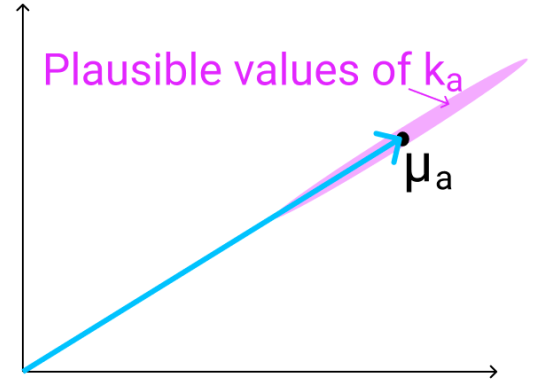
\includegraphics[scale=0.5]{figure1.png}
  \caption{The vector $\vmu_a$ (shown here in 2D as an example), with the range of possible values of $\vk_a$ shown in red. As mentioned previously, $\vk_a$ points in roughly the same direction as $\vmu_a$, but may have larger or smaller magnitude.}
  \label{fig:1}
\end{figure}

解: 定性来说, 不同采样得到的 $\vc$ 有很大的差别. 由 $\mSigma_{a}=\alpha \mi+\frac{1}{2}\vmu_{a} \vmu_{a}^{\top}$ 及 图 \ref{fig:1} 可知 $\vk_a$ 的方向近似为 $\vmu_a$ 的方向, $\vk_a$ 的长度大多数情况位于以下区间
\begin{equation}
  \|\vk_a\|\in[1-\beta,~1+\beta],\quad\beta\in(0,1)
\end{equation}

由 i. 可知 $\vq=M(\vmu_a+\vmu_b)$, 则 $\vk_a$ 注意力权重为
\begin{equation}
  \begin{aligned}
    \alpha_a
    &=\frac{\exp(\vk_{a}^{\top}\vq)}{\sum_{j=1}^{n}\exp(\vk_{j}^{\top}\vq)}\\
    &\in\left[\frac{\exp((1-\beta)M)}{\exp((1-\beta)M)+\exp(M)+n-2},~\frac{\exp((1+\beta)M)}{\exp((1+\beta)M)+\exp(M)+n-2}\right]\\
    &\approx[0,1]\\
  \end{aligned}
\end{equation}

$\vk_b$ 注意力权重为
\begin{equation}
  \begin{aligned}
    \alpha_b
    &=\frac{\exp(\vk_{b}^{\top}\vq)}{\sum_{j=1}^{n}\exp(\vk_{j}^{\top}\vq)}\\
    &\in\left[\frac{\exp(M)}{\exp((1+\beta)M)+\exp(M)+n-2},~\frac{\exp(M)}{\exp((1-\beta)M)+\exp(M)+n-2}\right]\\
    &\approx[0,1]\\
  \end{aligned}
\end{equation}

则由
\begin{equation}
  \vc\approx\alpha_a\vv_a+\alpha_b\vv_b
\end{equation}

可知 $\vc$ 与 $\vk_a$ 的长度大小有非常强的关联, 当 $\vk_a$ 的长度发生变化时, $\vc$ 也会发生很大的变化.

(d) \textbf{Benefits of multi-headed attention:} Now we'll see some power of multi-headed attention. We'll consider a simple version of multi-headed attention which is identical to single-headed self-attention as we've presented it in this homework, except two query vectors ($\vq_1$ and $\vq_2$) are defined, which leads to a pair of vectors ($\vc_1$ and $\vc_2$), each the output of single-headed attention given its respective query vector. The final output of the multi-headed attention is their average, $\frac{1}{2}(\vc_{1}+\vc_{2})$. As in question (c), consider a set of key vectors $\{\vk_{1},\vk_2,\dots, \vk_{n}\}$ that are randomly sampled $\vk_{i} \sim \mathcal{N}(\vmu_{i}, \mSigma_{i})$, where the means $\vmu_i$ are known to you, but the covariances $\mSigma_{i}$ are unknown. Also as before, assume that the means $\vmu_i$ are mutually orthogonal; $\vmu_{i}^{\top} \vmu_{j}=0$ if $i \neq j$, and unit norm, $\|\vmu_{i}\|=1$.

\quad i. Assume that the covariance matrices are $\mSigma_{i}=\alpha \mi$, for vanishingly small $\alpha$. Design query vectors $\vq_1$ and $\vq_2$ in terms of the $\vmu_i$ such that $\vc$ is \emph{approximately} equal to $\frac{1}{2}(\vv_{a}+\vv_{b})$.

\emph{Hint}: For the convenience of further analysis, you'd better recall the copy operation in question (a).

解: 令 $\vq_1=M\vmu_a$, $\vq_2=M\vmu_b$, 由协方差矩阵 $\mSigma_{i}=\alpha \mi$ 可知 $\vk_i\approx\vmu_i$, 则 $\vk_a$ 相对 $\vq_1$ 注意力权重为
\begin{equation}
  \alpha_a
  =\frac{\exp(\vk_{a}^{\top}\vq_1)}{\sum_{j=1}^{n}\exp(\vk_{j}^{\top}\vq_1)}
  \approx1
\end{equation}

则对 $\vq_1$ 输出
\begin{equation}
  \vc_1
  =\sum_{i=1}^{n}\alpha_{i}\vv_{i}
  \approx\vv_a
\end{equation}

$\vk_b$ 相对 $\vq_2$ 注意力权重为
\begin{equation}
  \alpha_b
  =\frac{\exp(\vk_{b}^{\top}\vq_2)}{\sum_{j=1}^{n}\exp(\vk_{j}^{\top}\vq_2)}
  \approx1
\end{equation}

则对 $\vq_2$ 输出
\begin{equation}
  \vc_2
  =\sum_{i=1}^{n}\alpha_{i}\vv_{i}
  \approx\vv_b
\end{equation}

所以
\begin{equation}
  \vc=\frac{1}{2}(\vc_{1}+\vc_{2})\approx\frac{1}{2}(\vv_{a}+\vv_{b})
\end{equation}

\quad ii. Assume that the covariance matrices are $ \mSigma_{a}=\alpha\mi+\frac{1}{2}\left(\vmu_{a} \vmu_{a}^{\top}\right) $ for vanishingly small $\alpha$, and $\mSigma_{i}=\alpha \mi$ for all $i \neq a$. Take the query vectors $\vq_1$ and $\vq_2$ that you designed in part i. What, qualitatively, do you expect the vector $\vc$ will look like for different samples? Please briefly explain why. You can ignore cases in which $\vk_{a}^{\top}\vq_{i}<0$.

解: 定性来说, 不同采样得到的 $\vc$ 几乎相同. 由 $\mSigma_{a}=\alpha \mi+\frac{1}{2}\vmu_{a} \vmu_{a}^{\top}$ 及 图 \ref{fig:1} 可知 $\vk_a$ 的方向近似为 $\vmu_a$ 的方向, $\vk_a$ 的长度多数情况位于以下区间
\begin{equation}
  \|\vk_a\|\in[1-\beta,~1+\beta],\quad\beta\in(0,1)
\end{equation}

忽略 $\vk_{a}^{\top}\vq_1<0$ 的情况, 由 $\vq_1=M\vmu_a$ 可知 $\vk_a$ 相对 $\vq_1$ 注意力权重为
\begin{equation}
  \alpha_a
  =\frac{\exp(\vk_{a}^{\top}\vq_1)}{\sum_{j=1}^{n}\exp(\vk_{j}^{\top}\vq_1)}
  \approx\frac{\exp(\|\vk_a\|M)}{\exp(\|\vk_a\|M)+n-1}
  \approx1
\end{equation}

$\vk_b$ 相对 $\vq_2$ 注意力权重没有变化, 仍然为
\begin{equation}
  \alpha_b
  =\frac{\exp(\vk_{b}^{\top}\vq_2)}{\sum_{j=1}^{n}\exp(\vk_{j}^{\top}\vq_2)}
  \approx1
\end{equation}

注意到 $\alpha_a\approx1$ 与 $\vk_a$ 的长度几乎无关, 则不同的采样仍然都会得到
\begin{equation}
  \vc\approx\frac{1}{2}(\vv_{a}+\vv_{b})
\end{equation}

(e) \textbf{Visualization:} Use the computer to sample 2-dimension key vectors multiple times and visualize the distributions of the output $\vc$ of query $\vq$ designed in (c) and (d) under different covariance matrices conditions. More specifically, we set $n = d = 2$, $\vv_1 = \vmu_{1} = (0, 1)^\top$ and $\vv_2 = \vmu_{2} = (1, 0)^\top$. You may have to carefully choose $\alpha$ to produce the desired phenomenon, we recommend $\alpha = 1\times10^{-10}$. Does this small experiment verify your findings in the above questions?

解: 这个小的数值实验可以验证上述题目的分析结果. 对键向量 $\{\vk_1,\vk_2\}$ 随机采样 10 次, 得到 (c) 题的可视化结果如图 \ref{fig:ci} 和 \ref{fig:cii} 所示.

\begin{figure}[htbp]
  \centering
  \begin{minipage}[t]{0.48\textwidth}
    \centering
    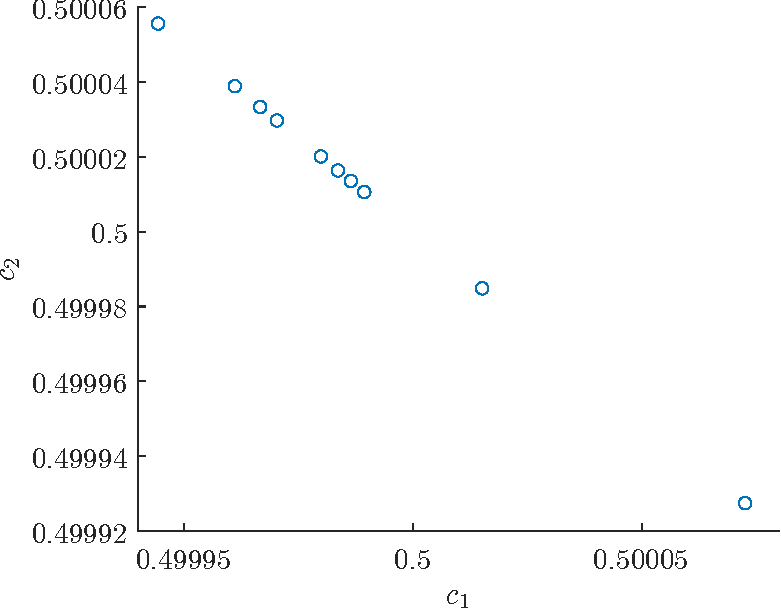
\includegraphics[width=8cm]{ci.pdf}
    \caption{(c) i. 注意力机制输出结果 $\vc$}
    \label{fig:ci}
  \end{minipage}
  \begin{minipage}[t]{0.48\textwidth}
    \centering
    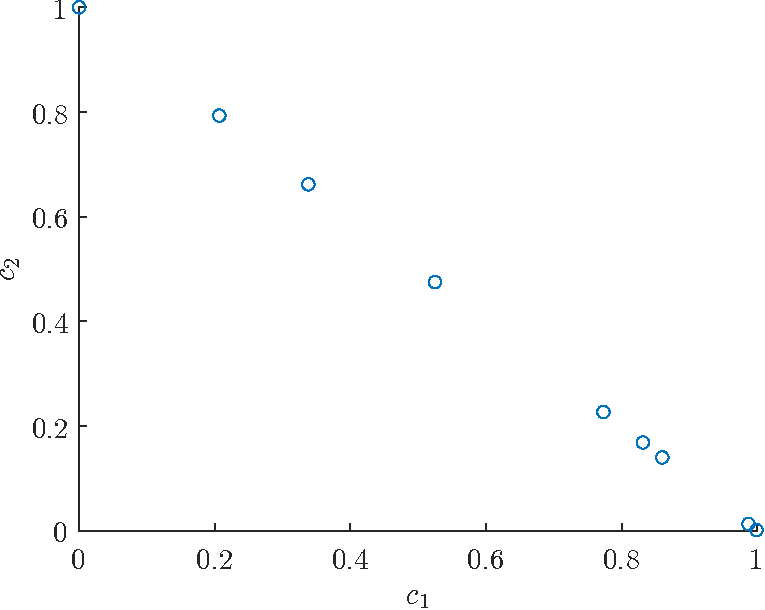
\includegraphics[width=8cm]{cii.pdf}
    \caption{(c) ii. 注意力机制输出结果 $\vc$}
    \label{fig:cii}
  \end{minipage}
\end{figure}

由图 \ref{fig:ci} 可知, 对单向 (single-headed) 注意力机制而言, 当 $\mSigma_{i}=\alpha \mi$ 时, 输出的结果都是 $\vc\approx\frac{1}{2}(\vv_{1}+\vv_{2})$; 由图 \ref{fig:cii} 可知, 当 $\mSigma_{1}=\alpha \mi+\frac{1}{2}\vmu_{1} \vmu_{1}^{\top}$ 时, 输出结果 $\vc$ 是 $\vv_1$ 与 $\vv_2$ 的任意凸组合.

(d) 题的可视化结果如图 \ref{fig:di} 和 \ref{fig:dii} 所示. 
\begin{figure}[htbp]
  \centering
  \begin{minipage}[t]{0.48\textwidth}
    \centering
    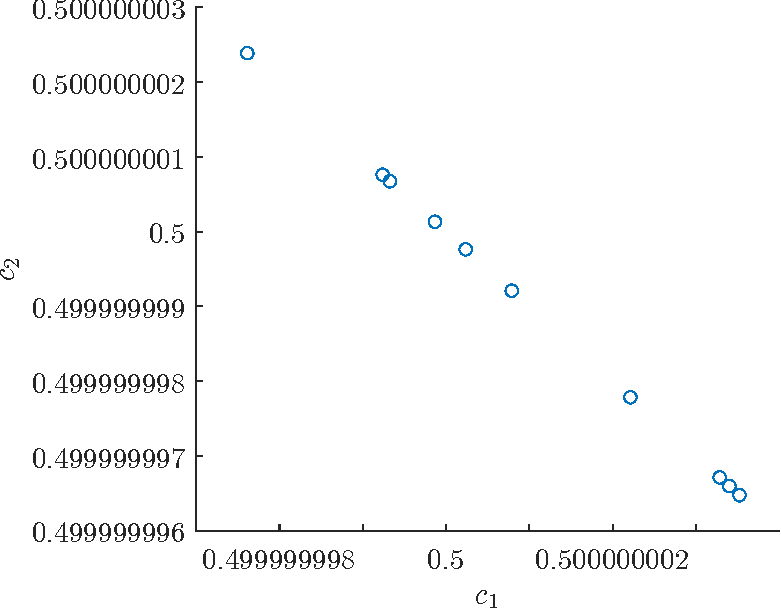
\includegraphics[width=8cm]{di.pdf}
    \caption{(d) i. 注意力机制输出结果 $\vc$}
    \label{fig:di}
  \end{minipage}
  \begin{minipage}[t]{0.48\textwidth}
    \centering
    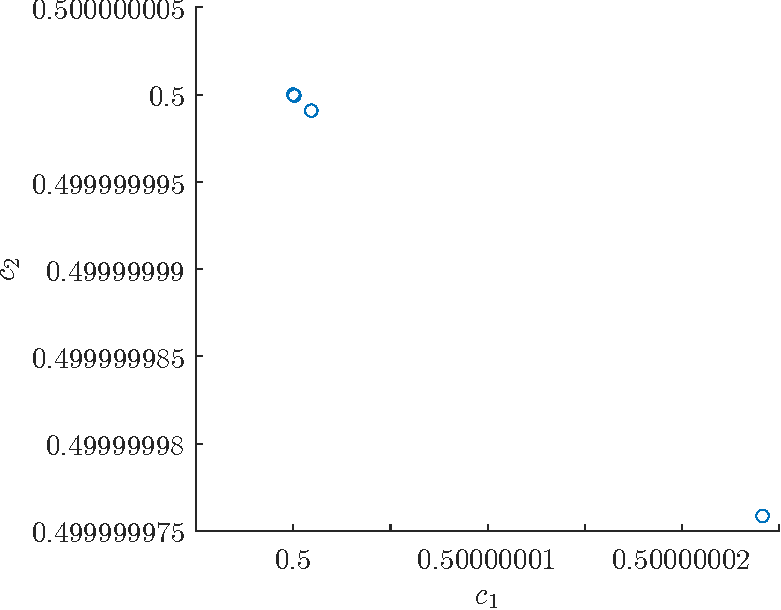
\includegraphics[width=8cm]{dii.pdf}
    \caption{(d) ii. 注意力机制输出结果 $\vc$}
    \label{fig:dii}
  \end{minipage}
\end{figure}

由图 \ref{fig:di} 可知, 对多向 (multi-headed) 注意力机制而言, 当 $\mSigma_{i}=\alpha \mi$ 时, 输出的结果都是 $\vc\approx\frac{1}{2}(\vv_{1}+\vv_{2})$; 由图 \ref{fig:dii} 可知, 当 $\mSigma_{1}=\alpha \mi+\frac{1}{2}\vmu_{1} \vmu_{1}^{\top}$ 时, 忽略 $\vk_{1}^{\top}\vmu_1<0$ 的情况, 输出的结果也是 $\vc\approx\frac{1}{2}(\vv_{1}+\vv_{2})$, 不受协方差矩阵 $\mSigma_{1}$ 变化的影响, 即若 $\vk_1$ 只是大小发生变化而方向几乎不变则对输出 $\vc$ 几乎没有影响.

\section*{Programming: Natural Language Processing (NLP)}

4. Please install \href{https://pytorch.org/}{PyTorch}, \href{https://jupyter.org/install}{Jupyter Notebook} and run the \href{https://pytorch.org/tutorials/_downloads/a60617788061539b5449701ae76aee56/seq2seq_translation_tutorial.ipynb}{NLP tutorial}. If you want to use TensorFlow or other deep learning frameworks, please find corresponding language translation tutorial for that framework and run it. The tutorial is the third example for NLP From Scratch in \href{https://pytorch.org/tutorials/index.html}{Pytorch tutorials}, where we write our own classes and functions to preprocess the data to do NLP modeling tasks. We hope after you complete this tutorial that you'll proceed to learn how torchtext can handle much of this preprocessing for you in the three tutorials immediately following this one. In this project we will be teaching a neural network to translate from French to English. The code is given as a jupyter notebook file. 

All you need to do is to read, run and think. You need not write any code or any report in this programming.

% Reference
\begin{thebibliography}{1}

\bibitem{udlstm}
Olah, Chris. Understanding LSTM Networks, 2015. 

\url{http://colah.github.io/posts/2015-08-Understanding-LSTMs/}.


\end{thebibliography}

\end{document}
